\begin{frame}
  \titlepage
\end{frame}


\section{Introdução}
\begin{frame}{Introdução}
    
    \begin{block}{Problema}
        Ambiente parcialmente observável\\
        \pause
        Inviável uso de planejamento clássico
    \end{block}
    \pause
    \begin{block}{Solução}
        Planejadores conformantes
    \end{block}
    \pause
    \begin{block}{Nova abordagem}
        \[ \text{Traduções} + \text{Planejador Clássico} \]
    \end{block}

\end{frame}


\section{Planejamento clássico}
\begin{frame}{Definição}
    \begin{block}{Problema de planejamento clássico}
        Criar um plano de ações para atingir as metas a partir de um estado 
inicial conhecido \cite{Ghallab:2004}. \\
        \begin{center}
            $P = \langle S, s_0, S_G, A, f \rangle$
        \end{center}
    \end{block}
    
\end{frame}
\begin{frame}{Exemplo}
    
    \begin{align*}
            F  \quad  & In(A),In(B),Dirt(A),Dirt(B) \\
            A  \quad  & D: \text{Prec} = \emptyset, Ef= \{ In(A) \rightarrow In(B),\lnot In(A) \} \\
                      & E: \text{Prec} = \emptyset, Ef= \{ In(B) \rightarrow In(A),\lnot In(B) \} \\
                      & A: \text{Prec} = \emptyset, Ef= \{ In(A)  \rightarrow \lnot Dirt(A); In(B) \rightarrow \lnot Dirt(B) \} \\
           s_0 \quad  & \{ In(A), Dirt(A), Dirt(B)  \} \\
           G   \quad  & \{ \lnot Dirt(A),\lnot Dirt(B)  \} \\
    \end{align*}
    
    $\pi = (A,D,A)$
    
    $\lnot Dirt(A)$
\end{frame}



\begin{frame}{Suposições Restritivas \footnote{\cite{Ghallab:2004}}}
    \begin{enumerate}
        \item Espaço de estados finito 
        \item Ambiente totalmente observável \label{A:1}
        \item Função de transição determinística 
        \item Ambiente estático (sem agentes externos)
        \item Existem apenas metas de alcançabilidade 
        \item Planos sequenciais
        \item Tempo implícito
        \item Planejamento \textit{off-line}
    \end{enumerate}
    
\end{frame}

\begin{frame}{Extensão do problema}
    \begin{block}{Relaxar a suposição \ref{A:1} Ambiente totalmente observável}
        Ambiente sem observação e incerteza no estado inicial
    \end{block}
    
    \begin{block}{Nova Extensão}
        Problema de Planejamento Conformante
    \end{block}
    \pause
    \begin{block}{Problema de planejamento clássico}
        \begin{center}
            $P = \langle S, s_0, S_G, A, f \rangle$
        \end{center}
    \end{block}
    
    \begin{block}{Problema de planejamento conformante}
        \begin{center}
            $P = \langle S, S_0, S_G, A, f \rangle$
        \end{center}
    \end{block}
\end{frame}




\section{Planejamento Conformante}
%\subsection{Definição}

\begin{frame}{Definição}
    \begin{block}{Planejamento Conformante}
    {  Planejamento com informação incompleta e \textbf{sem sensoreamento}. Em 
    que uma meta deve ser atingida apesar da incerteza no estado inicial.}
    \end{block}

    { \small Uma solução para o problema de planejamento conformante é uma sequência de ações 
    que mapeia todos os possíveis estados iniciais em algum estado meta.} \\
    \pause
    \begin{block}{ \alert{\bf Desafios}}
        \begin{itemize}
         \item representar crenças
         \item encontrar heurísticas eficientes para o \textbf{espaço de crenças}
        \end{itemize}
    
    \end{block}

\end{frame}

\begin{frame}{Espaço de busca}
    \begin{block}{Estados de crença}
    { Quando o mundo é parcialmente observável, o estado de crenças 
representa o conjunto de possíveis estados onde o agente pode se encontrar. } \\
    \end{block}
    
    \begin{block}{Tamanho}
        \begin{itemize}
        \item O espaço de crença é composto de todas as possíveis combinações de 
    estados físicos.

        \item Seja $n = |S|$ o número de estados do problema, há $2^{\textit{n}}$ possíveis 
        estados de crença.\\
        
        \item NP-Completo
        %\item Para $n$ grande, é difícil manter todos os estados de crença.
        \end{itemize}
    \end{block}
   
\end{frame}

\begin{frame}{Espaço de busca (Clássico vs Conformante)}

    \begin{multicols}{2}
        \centering
    
        Espaço de Estados: \footnote{\cite{AIMA2013}}
        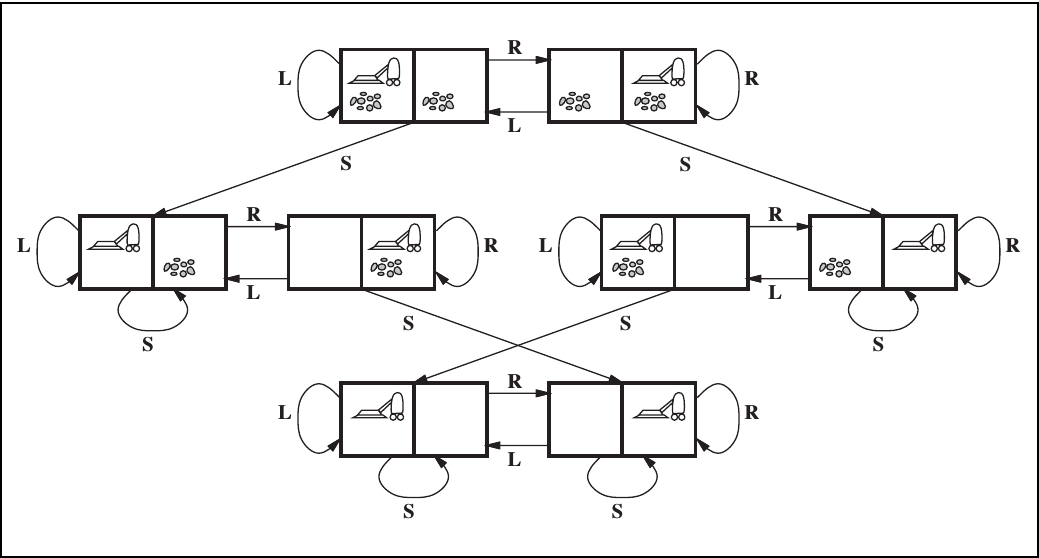
\includegraphics[scale=0.2]{images/space_of_states.png}
    \columnbreak
    
        Espaço de Crenças Reduzido:
        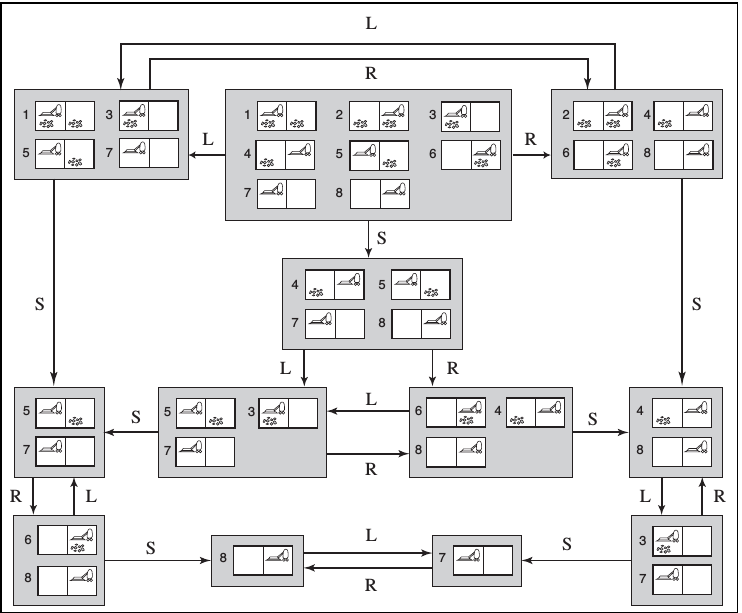
\includegraphics[scale=0.28]{images/belief_space.png}
    \end{multicols}
    
\end{frame}


% \subsection{Complexidade}
% \begin{frame}{Planejamento conformante}
% \begin{itemize}
%  \item O planejamento conformante é um problema de busca em espaço de crenças em 
% lugar de espaço de estados.
%  \item O espaço de crenças pode chegar a ser de tamanho exponencial no numero de 
% estados. 
%  \item O planejamento clássico é NP-Completo, mas o planejamento conformante é 
% mais difícil
% \end{itemize}
% \end{frame}
% 
% \begin{frame}{Planejamento conformante}
% \begin{figure}
% %\includegraphics[scale=0.45]{beliefSpace.png}
% \end{figure}
% 
% \end{frame}


\begin{frame}{Modelo}
Formalmente o planejamento conformante pode ser caracterizado por uma tupla 
$S=\langle S, S_0, S_G, A, f \rangle$, sendo:
\begin{itemize}
\item $S$ é um espaço finito de estados,
\item $S_0$ é um conjunto não vazio de possíveis estados iniciais $S_0\subseteq 
S$,
\item $S_G$ é um conjunto não vazio de estados meta $S_G \subseteq S$,
\item $A$ é um conjunto de ações em que $A(s)$ denota o conjunto de ações 
aplicáveis no estado $s \in S$ e
\item $f$ é uma função de transição de estados não-determinística, em que 
$f(a,s)$ indica o conjunto não-vazio de possíveis estados sucessores de $s$, que 
são obtidos aplicando a ação $a \in A(s)$ em s.
\end{itemize}
\end{frame}


\begin{frame}{Sintaxe}
Um problema de planejamento é definido pela seguinte tupla: $P=\langle F, I, O, G\rangle$, 
onde:
\begin{itemize}
 \item $F$ é o conjunto de proposições do problema.
 \item $I$ é o conjunto de cláusulas sobre $F$ que definem a situação inicial.
 \item $O$ é o conjunto das ações. Cada ação $a$, tem uma precondição $Pre(a)$ 
$\subseteq F$, e um conjunto de efeitos condicionais: $C\rightarrow E_1 \mid ... 
\mid E_n$, sendo $C\subseteq F$ e $E_i \subseteq F$. (Se $n > 1$ é 
não-determinístico). 
 \item $G$ é o sub-conjunto de $F$ que define o estado meta. 
\end{itemize}

\end{frame}


\begin{frame}{Semântica}
    Um problema de planejamento conformante define um modelo de estados $S(P) = \langle S, S_0, S_G, A, F\rangle$:
    \begin{itemize}
        \item $S$ é o conjunto de possíveis valores das proposições em $F$.
        \item $S_0$ e $S_G$ é o conjunto de possíveis valores que satisfazem $I$ e $G$.
        \item $O(s)$ é o conjunto de operadores, as precondições dos quais são 
            verdadeiras em $s$.
        \item $f(a,s)$ é a função de transição não-determinística que resulta de obter 
            os estados sucessores que seguem a ação $a$, no estado $s$.
    \end{itemize}
    Um plano conformante para $P$, é um plano conformante para $S(P)$.
\end{frame}



\begin{frame}{Exemplo}
    Aspirador com incerteza na posição
    \begin{itemize}
        \item $F = \{A,L_A,L_B\}$.
        \item $I $ te 
        \item $O $ te
        \item $G $ e
    \end{itemize}

\end{frame}




\section{Tradução $K_0$}

\begin{frame}{Proposta}
    \begin{itemize}
    \item Substituir cada literal $L$ por $ KL$ ou $K \lnot L$
    \item Utilizar um planejador clássico para resolver o problema
    \end{itemize}  
\end{frame}

\begin{frame}{Definição do problema traduzido}

    Dado um problema de planejamento conformante:\\
    $P=\langle F, I, O, G\rangle$,
    
    podemos definir um problema clássico equivalente:\\
    $K_0(P)=\langle F', I', O', G'\rangle$
    \begin{itemize}
        \item $F' = \{ KL, K \lnot L | L \in F \}$
        \item $I' = \{ KL | L \in I \}$
        \item $G' = \{ KL | L \in G \}$
%         \item $O' = O$, substituindo $L$ por $KL$ e para cada efeito condicional substui-se
        $C \rightarrow L$ por $KC \rightarrow KL$ e $\lnot K \lnot C \rightarrow \lnot K \lnot C$. 
    \end{itemize}  
\end{frame}



\begin{frame}{Exemplo}
    
\end{frame}

\begin{frame}{Características}
    \begin{block}{CORRETO}
        Todo plano que resolve $K_0(P)$ resolve $P$
    \end{block}
    \begin{block}{Não é COMPLETO}
        Existem problemas conformantes com solução que ele não encontra
    \end{block}
    
    
\end{frame}

\section{Tradução $K_{T,M}$}


\begin{frame}{Traduções para planejamento Conformante}
\begin{itemize}
\item O problema conformante $P$, é traduzido numa versão clássica do mesmo 
problema: $K_{T,M}(P)$. 
\item A tradução $K$ é a versão epistêmica do problema $P$, que significa que 
raciocinaremos sobre o conhecimento que temos dos literais em $P$.
\item O significado do \textit{operador} $K$ é indicar se a variável $L$ e 
conhecida. Por exemplo $KL$ significa que sabemos que o valor de $L$ é verdade, 
e $K \lnot L$ que sabemos que $L$ é falso.
\item Similarmente para $\lnot KL$ não sabemos se o valor de $L$ é verdadeiro, e 
$\lnot K \lnot L$ não sabemos se $L$ é falso. Assim eliminamos toda incerteza na 
situação inicial em $K(P)$ %\cite{palacios2007conformant}.
\end{itemize}  
\end{frame}

\subsection{Tags e Merges}
\begin{frame}{Traduções para planejamento Conformante}
\begin{itemize}
\item $T$ e $M$ são dois parâmetros, o conjunto de \textit{tags} e o conjunto de 
\textit{merges}. 
\item Um \textit{tag} $t \in T$ é um conjunto de literais $L$ de $P$, do qual 
não conhecemos o valor no estado inicial $I$. 
\item A operação de \textit{merge} permite obter conhecimento sobre literais. 
Cada operação de \textit{merge} é uma dupla $(R,L) \in M$ que contem o conjunto 
de tags $R \subseteq T$, e o literal $L$ de $P$. 
\item Uma operação de \textit{merge} é valida quando um dos \textit{tags} $t$ é 
verdadeiro no estado inicial $I$. 
\end{itemize}
\begin{equation*}
I \models \bigvee_{t \in R} t.
\end{equation*}
\end{frame}

\begin{frame}{Traduções para planejamento Conformante}
\begin{itemize}
\item Os \textit{tags} são assunções sobre o estado inicial, um deles tem que 
ser verdadeiro no estado inicial.
\item A operação de \textit{merge} nos da o conhecimento sobre o valor do 
literal $L$, quando tivermos o valor $L$ conhecido para todos os diferentes 
\textit{tags}:
\end{itemize}
\begin{equation*}
m_{R,L} : \bigwedge_{t \in R} KL/t \rightarrow KL.
\end{equation*}
\end{frame}

\subsection{Tradução}
\begin{frame}{Traduções para planejamento Conformante}
Para o problema $P=\langle F, O, I, G\rangle$ definimos a tradução $K_{T,M}(P) = 
\langle F', O', I', G'\rangle$ como:
\begin{itemize}
\item $F' = \lbrace KL/t, K\lnot L/t \vert L \in F \quad e \quad t \in T 
\rbrace$
\item $I' = \lbrace KL/t, \vert$ se $I \models t \supset L  \rbrace$ 
\item $G' = \lbrace KL \vert L \in G \rbrace$
\item $O' = \lbrace a: KC/t \rightarrow KL/t, a: \lnot K \lnot C / t \rightarrow 
\lnot K \lnot L/t \vert a: C \rightarrow L$ in $P \rbrace \cup \lbrace m_{R,L} 
\rbrace$ 
\end{itemize}
\end{frame}

\subsection{Exemplos}
\begin{frame}{Exemplo}
    \begin{multicols}{2}
        \centering
        
        %\includegraphics[scale=0.2]{grid.jpg}\\
    \columnbreak
        \begin{itemize}
        \item $F = \lbrace On_{x,y} \rbrace$
        \item $I=\lbrace On_{1,5}, On_{1,6}, On_{2,5}, On_{2,6} \rbrace$
        \item $A=\lbrace moveRight(), moveLeft(),$ $moveUp(), moveDown() 
\rbrace$
        \item $G=\lbrace On_{6,1}\rbrace$.
        \end{itemize} 
    \end{multicols}
\end{frame}

\begin{frame}{Exemplo}
    A tradução do problema anterior $K_{T,M}(P) = \langle F', O', I', 
G'\rangle$:
    \begin{itemize}
    \item O conjunto $T$ de \textit{tags}, que incluiria os possíveis estados 
iniciais: 
    $t_1 = On_{1,5}, t_2 = On_{1,6}, t_3 = On_{2,5}, t_4 = On_{2,6}$.
    \item $F = \lbrace  K \lnot On_{1,1} / t_1, K \lnot On_{1,1} / t_2,$ 
    $ K \lnot On_{1,1} / t_3, K \lnot On_{1,1} / t_4, K \lnot On_{1,2} / t1,... 
\rbrace$
    \item $I=\lbrace K On_{1,5}/t_1, K On_{1,6}/t_2, K On_{2,5}/ t_3, K 
On_{2,6}/ t_4 \rbrace$
    \item $G=\lbrace K On_{6,1}\rbrace$.
    \end{itemize}
\end{frame}


\subsection{Conclusão}
\begin{frame}
    \begin{itemize}
        \item O 
    \end{itemize}
\end{frame} 
